\documentclass{article}
\usepackage[margin=1in]{geometry}
\usepackage{inconsolata}
\usepackage{dirtytalk}
\usepackage{tikz}
\usepackage{float}
\usepackage{listings}
\usepackage{hyperref}
\usepackage{pgfplots}

\usetikzlibrary{automata}

\title{COMS 4995 Final Project}
\author{Zehua Chen (zc2616)}
\date{\today}

\lstset{
  basicstyle=\footnotesize\ttfamily,
  numbers=left
}

\pgfplotsset{width=0.7\textwidth,compat=1.9}

\newcommand{\code}[1]{{\ttfamily #1}}

\begin{document}
  \maketitle
  \tableofcontents

  \setlength{\parskip}{8px}
  \setlength{\parindent}{0px}

  \section{Implementation}

    \subsection{Coordinate System}

      The world has a height and a width. The origin (0, 0) is located at the
      center of the world. If we save the world as an image, positive
      axis would be on the right of the image and positive y axis
      would be on the top of the image.

      In order for a cell to exist at (0, 0) and the world be modeled using
      width and height, width and height must be odd numbers

    \subsection{Single Core}

      Single core implementation (\code{Conway.Simulate.simulateSync})
      of the simulation:

      \begin{enumerate}
        \item \label{single: step-simulate} Simulate the world
        \item \label{single: step-grow} Simulate one layer outside of the existing world, and expand
        the existing world if needed
      \end{enumerate}

    \subsection{Multi Core}

      Multicore implementation (\code{Conway.Simulate.simulateAsync})
      of the simulation

      \begin{enumerate}
        \item \label{multi: step-partition}
        Divide the world into partitions and calculate adjacent cells
        between partitions
        \item \label{multi: step-simulate}
        Simulate the partitions, with access only to the world within the
        partition. \emph{This step reuses code of step \ref{single: step-simulate} from
        single core implementation}
        \item \label{multi: step-simulate-border}
        Simulate the adjacent cells between partitions, with access to the
        whole world.
        \item \label{multi: step-grow}
        Simulate one layer outside of the existing world. \emph{This step reuses
        code of step \ref{single: step-simulate} from single core implementation}
        \item Combine the result of \ref{multi: step-simulate},
        \ref{multi: step-simulate-border} and \ref{multi: step-grow}
      \end{enumerate}

      Of the above steps, the operations are \ref{multi: step-partition}
      is performed in parallel first. After they finish, the operations in
      \ref{multi: step-simulate}, \ref{multi: step-simulate-border},
      \ref{multi: step-grow} are performed in parallel. The latter operations
      are performed in a second step because they depend on the result from
      the former operations.

      \subsubsection{Parameters}

        Multicore simulation allows customizations in

        \begin{itemize}
          \item slice width, slice height: how big each slice should be
          \item chunk size: the multi core simulation uses \code{parList} in
          some operations. Chunk size is used to customize \code{parList}
        \end{itemize}

    \subsection{Modules}

      \begin{enumerate}
        \item \code{Conway.World}: provide abstraction to the conway world,
        and various utility functions useful for operations on the world
        \item \code{Conway.Slice}: provide abstraction of slices of worlds
        \item \code{Conway.Partition}: provide function that split the world
        into slices, and find the cells on the outer layer of each partition
        \item \code{Conway.Simulate}: implements single and multi core
        simulation
        \item \code{Conway.PPM}: saves a conway world into a PPM image
      \end{enumerate}

    \subsection{Testing}

      \begin{enumerate}
        \item \code{test/World.hs}: tests for \code{Conway.World}
        \item \code{test/Partition/Partition.hs}: make sure the world can be
        divided into partitions
        \item \code{test/Partition/PartitionBorders.hs}: make sure the outer
        most layer of a partition can be resolved property
        \item \code{test/Simulate/Finite.hs}: make sure that simulation on
        finite grid is correct
        \item \code{test/Simulate/Grow.hs}: make sure that teh grid is grown
        when needed
        \item \code{test/Simulate/Infinite.hs}: make sure that single core
        and multi core implementation produces the same result from simulating
        on an infinite grid.
      \end{enumerate}

    \subsection{Command Line Interface}

      \subsubsection{Simulation}

        In order to run simulation, pass the following to the command line application

        \begin{lstlisting}
conway-exe <file> <iterations> <slice width> <slice height> <chunk size>
        \end{lstlisting}

        \say{file} is a json file containing the description of the world. The
        file should look like the following.

        \lstinputlisting{../sample-input.json}

        After the simulation has finished, the program will save two
        images \code{sync.ppm} and \code{async.ppm}, one produced by
        single core simulation, and the other produced by multi core simulation.

      \subsubsection{Benchmarking}

        In order to benchmark, give the following to the command line application

        \begin{lstlisting}
conway-exe benchmark
        \end{lstlisting}

  \section{Performance}

    My machine has the following specs

    \begin{itemize}
      \item 2 energy efficient cores
      \item 6 performance cores
      \item 16 GB of memory
    \end{itemize}

    Benchmarking is done using \code{Criterion.Main}

    \subsection{Single Iteration on World of Size 101 x 101}

      \begin{figure}[H]
        \centering
        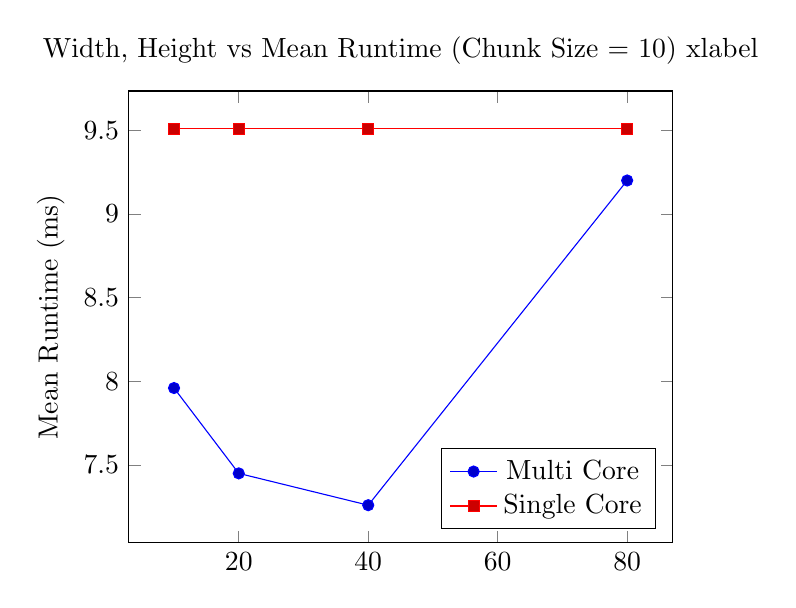
\begin{tikzpicture}
          \begin{axis}[
            title={Width, Height vs Mean Runtime (Chunk Size = 10)}
            xlabel={Width, Height},
            ylabel={Mean Runtime (ms)},
            legend pos=south east
          ]
            \addplot coordinates { (10, 7.96) (20, 7.45) (40, 7.26) (80, 9.2)};
            \addlegendentry{Multi Core}

            \addplot coordinates { (10, 9.51) (20, 9.51) (40, 9.51) (80, 9.51)};
            \addlegendentry{Single Core}
          \end{axis}
        \end{tikzpicture}
      \end{figure}

      The above data is generated by changing the slice width and slice
      height of async simulation, while keeping chunk size at 10.

      \begin{figure}[H]
        \centering
        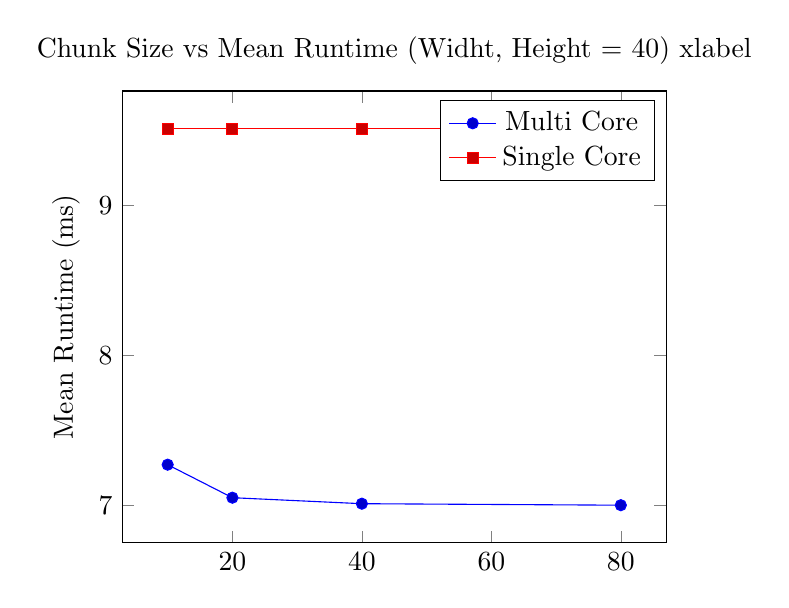
\begin{tikzpicture}
          \begin{axis}[
            title={Chunk Size vs Mean Runtime (Widht, Height = 40)}
            xlabel={Chunk size},
            ylabel={Mean Runtime (ms)}
          ]
            \addplot coordinates { (10, 7.27) (20, 7.05) (40, 7.01) (80, 7.00)};
            \addlegendentry{Multi Core}

            \addplot coordinates { (10, 9.51) (20, 9.51) (40, 9.51) (80, 9.51)};
            \addlegendentry{Single Core}
          \end{axis}
        \end{tikzpicture}
      \end{figure}

      The above data is generated by changing the chunk size while
      keeping slice width and slice height at 40

    \subsection{100 Iterations on World of Size 51 vs 51}

      \begin{figure}[H]
        \centering
        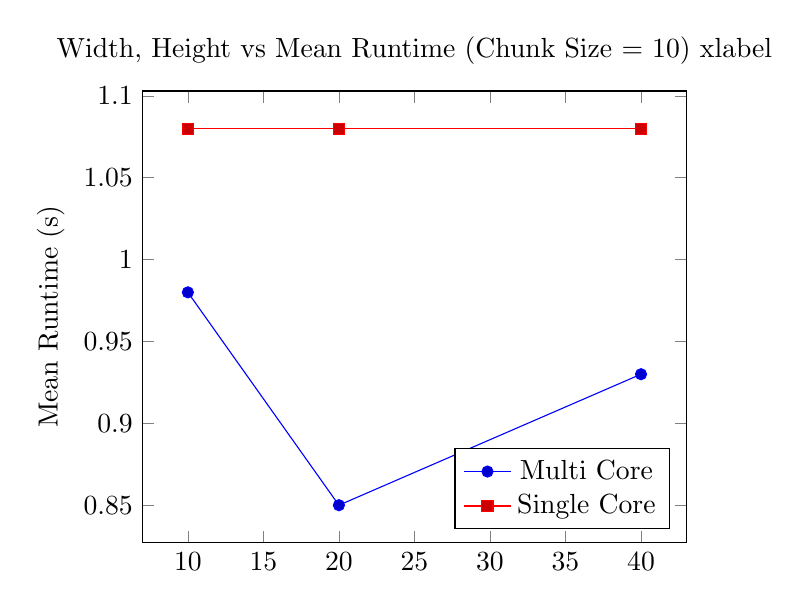
\begin{tikzpicture}
          \begin{axis}[
            title={Width, Height vs Mean Runtime (Chunk Size = 10)}
            xlabel={Width, Height},
            ylabel={Mean Runtime (s)},
            legend pos=south east
          ]
            \addplot coordinates { (10, 0.98) (20, 0.85) (40, 0.93)};
            \addlegendentry{Multi Core}

            \addplot coordinates { (10, 1.08) (20, 1.08) (40, 1.08)};
            \addlegendentry{Single Core}
          \end{axis}
        \end{tikzpicture}
      \end{figure}

      The above data is generated by changing the slice width and slice
      height of async simulation, while keeping chunk size at 10.

      \begin{figure}[H]
        \centering
        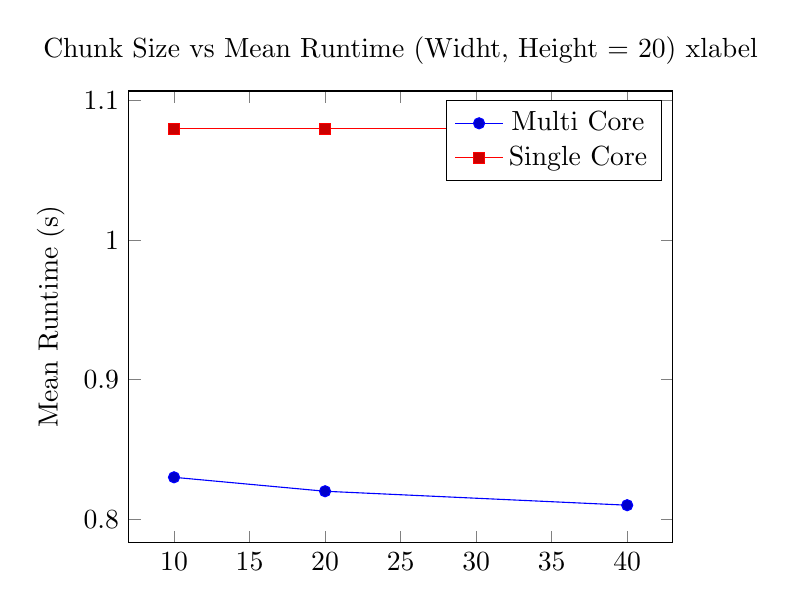
\begin{tikzpicture}
          \begin{axis}[
            title={Chunk Size vs Mean Runtime (Widht, Height = 20)}
            xlabel={Chunk size},
            ylabel={Mean Runtime (s)}
          ]
            \addplot coordinates { (10, 0.83) (20, 0.82) (40, 0.81)};
            \addlegendentry{Multi Core}

            \addplot coordinates { (10, 1.08) (20, 1.08) (40, 1.08)};
            \addlegendentry{Single Core}
          \end{axis}
        \end{tikzpicture}
      \end{figure}

      The above data is generated by changing the chunk size while
      keeping slice width and slice height at 20

    \subsection{Conclusion}

      From the above performance figures, the following can be concluded

      \begin{itemize}
        \item The multi core implementation takes around 80\% of the time
        it takes for single core implementations regardless of the number
        of iterations and world size
        \item Increasing chunk size can reduce performance
        \item Slice width and height needs tuning in order to achieve the
        best performance. On my machine the best slice width and height
        should be around half of the world width and height.
      \end{itemize}

  \section{Code}

    \subsection{Command Line Application}

      \lstinputlisting[caption=\code{Main.hs}]{../app/Main.hs}
      \lstinputlisting[caption=\code{Benchmark.hs}]{../app/Benchmark.hs}

    \subsection{Implementation}

      \lstinputlisting[caption=\code{Conway.Partition}]{../src/Conway/Partition.hs}
      \lstinputlisting[caption=\code{Conway.PPM}]{../src/Conway/PPM.hs}
      \lstinputlisting[caption=\code{Conway.Simulate}]{../src/Conway/Simulate.hs}
      \lstinputlisting[caption=\code{Conway.Slice}]{../src/Conway/Slice.hs}
      \lstinputlisting[caption=\code{Conway.World}]{../src/Conway/World.hs}

    \subsection{Testing}

      \lstinputlisting[caption=\code{test/World.hs}]{../test/World.hs}
      \lstinputlisting[caption=\code{test/Partition/Partition.hs}]{../test/Partition/Partition.hs}
      \lstinputlisting[caption=\code{test/Partition/PartitionBorder.hs}]{../test/Partition/PartitionBorder.hs}
      \lstinputlisting[caption=\code{test/Simulate/Finite.hs}]{../test/Simulate/Finite.hs}
      \lstinputlisting[caption=\code{test/Simulate/Grow.hs}]{../test/Simulate/Grow.hs}
      \lstinputlisting[caption=\code{test/Simulate/Infinite.hs}]{../test/Simulate/Infinite.hs}

\end{document}
